\documentclass[tikz,border=5pt]{standalone}

\begin{document}
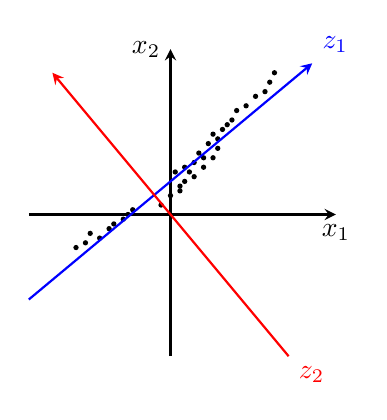
\begin{tikzpicture}[scale=0.6,>=stealth]

  % Axes
  \draw[thick,->] (-3,0) -- (3.5,0) node[below] {$x_1$};
  \draw[thick,->] (0,-3) -- (0,3.5) node[left] {$x_2$};

  % Scatter points (rough diagonal cluster)
  \foreach \x/\y in {
    % upper-right cloud
    0.2/0.6, 0.4/0.9, 0.5/1.1, 0.7/1.2, 0.8/1.5,
    1.0/1.6, 1.1/1.8, 1.3/2.0, 1.4/2.2, 1.6/2.3,
    1.8/2.5, 2.0/2.6, 2.1/2.8, 2.2/3.0,
    0.1/0.9, 0.3/1.0, 0.6/1.3, 0.9/1.7, 1.2/1.9,
    % central band
    -0.2/0.2, 0.0/0.4, 0.2/0.5, 0.3/0.7, 0.5/0.8,
    0.7/1.0, 0.9/1.2, 1.0/1.4,
    % lower-left small cloud
    -2.0/-0.7, -1.8/-0.6, -1.7/-0.4, -1.5/-0.5, -1.3/-0.3,
    -1.2/-0.2, -1.0/-0.1, -0.9/0.0, -0.8/0.1
  }{
    \fill (\x,\y) circle[radius=1.6pt];
  }

  % PCA axes
  % PC1: along the main diagonal direction (roughly slope ~1)
  \draw[ thick,blue,->] (-3,-1.8) -- (3,3.2) node[anchor=south west] {$z_1$};

  % PC2: perpendicular to PC1
  \draw[ thick,red,<-] (-2.5,3) -- (2.5,-3) node[anchor=north west] {$z_2$};

\end{tikzpicture}
\end{document}